\documentclass[floatfix]{article}  
\pagestyle{plain}

\usepackage{amsmath,amssymb}
\usepackage{dsfont}
\usepackage{graphicx} %loads the graphicx.sty package 
\usepackage{epstopdf} %loads the epstopdf.sty package 
\usepackage{slashed}
\usepackage{color}

\usepackage{graphicx,longtable,tocloft,color}
\usepackage{sidecap}
\usepackage{subfig}
\usepackage{xspace}
\usepackage{mydefs}
\usepackage{cite}
\usepackage{lineno}
\usepackage{multirow}
\usepackage{hyperref}
%\usepackage[left=2cm,right=2cm,top=2cm,bottom=2cm]{geometry}
%\tolerance = 1000
%\parindent 0cm
%\parskip 2mm
%
%
%for draft only:
%\linenumbers
\usepackage{array}

\title{Irreducible backgrounds and measurement uncertainties}

\author{Jonathan M. Butterworth$^1$, Vitaliano Ciulli, Paolo Francavilla,\\ Frank Krauss$^2$, Carlo Pandini, Luca Parrozzi \\
\it $^1$Department of Physics and Astronomy, University College London,\\ 
\it $^2$IPPP, Department of Physics, Durham University}

\begin{document}

\maketitle 

\begin{abstract}
\end{abstract}

\section{Introduction}
\label{sec:intro}

The general principle of minimising the model-dependence of results from particle colliders by making measurements of 
well-defined final states in fiducial regions is by now widely accepted, and implemented by the LHC collaborations. 
The fiducial regions are design to reflect  the acceptance of the detectors and data-selection. 
The final states are defined in terms of stable, or quasi-stable,
particles. Increasingly impressive theoretical calculations are able to implement the appropriate kinematic cuts, and
modulo some uncertainty associated with soft physics (for example hadronisation), can predict precisely what 
is actually being measured, without the need for additional assumptions or extrapolations into unmeasured regions of 
phase space.

This represents great progress. One area, however, where the principle of defining a measurement in terms of the final state
not so widely implemented, is in the consideration of background processes and their subtraction. 
Often backgrounds are subtracted using a mixture of theoretical and data-drived techniques, 
even though in some cases the backgrounds are strictly speaking ``irreducible'', in that they produce final states 
identical to the ``signal'' final state (even in a perfect detector) and thus should be added to the signal 
at the amplitude, rather than cross-section, level. These subtractions are also often carried out before, or intermingled with, 
the unfolding and correction for detector effects such as efficiency and resolution, and thus are impossible to
undo or redo after the fact. 

In practice, the uncertainty introduced by such subtractions is negligible compared to other uncertainties in the measurements, 
for example because the kinematic overlap
is in fact small and interference terms are negligible. Nevertheless, in some processes, and as precision of both experiment
and theory increase, such considerations may become important. In this contribute we highlight some such cases in an attempt 
to raise awareness of the issues for future studies. 

\section{Single top and $W+b$ production}

An example of a final state in which two contributions are often treated as distinct processes is the measurement of a leptonic
decaying $W$ boson (that is, charged lepton plus missing transverse energy) in association with a $b$-tagged hadronic jet. 
The publication of the ATLAS analysis of 7~TeV collision data\cite{Aad:2013vka} contains a measurement of the fiducial $W+b$ 
cross section both with and without the subtraction of the single-top contribution to the identical final state. Both
versions are available in HEPDATA~\cite{} and Rivet~\cite{Buckley:2010ar}. The unsubtracted version is show in Fig.~\ref{fig:wb}, 
and the subtracted version in Fig.~\ref{fig:notop}. 

\begin{figure}%[htbp!]
\centering
\subfloat{
	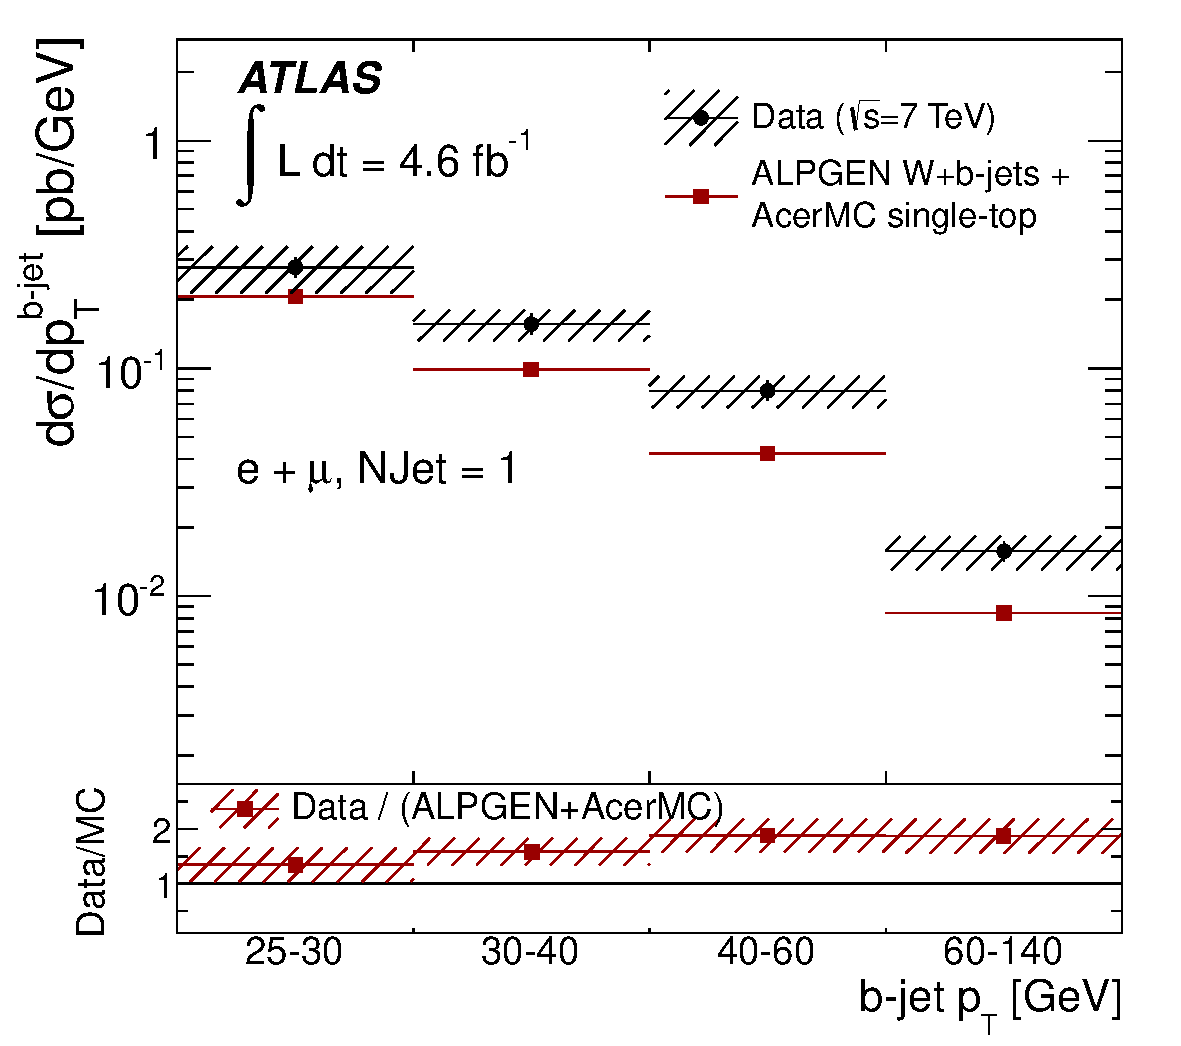
\includegraphics[width=0.48\textwidth]{fig_09a.pdf}
}
\subfloat{
	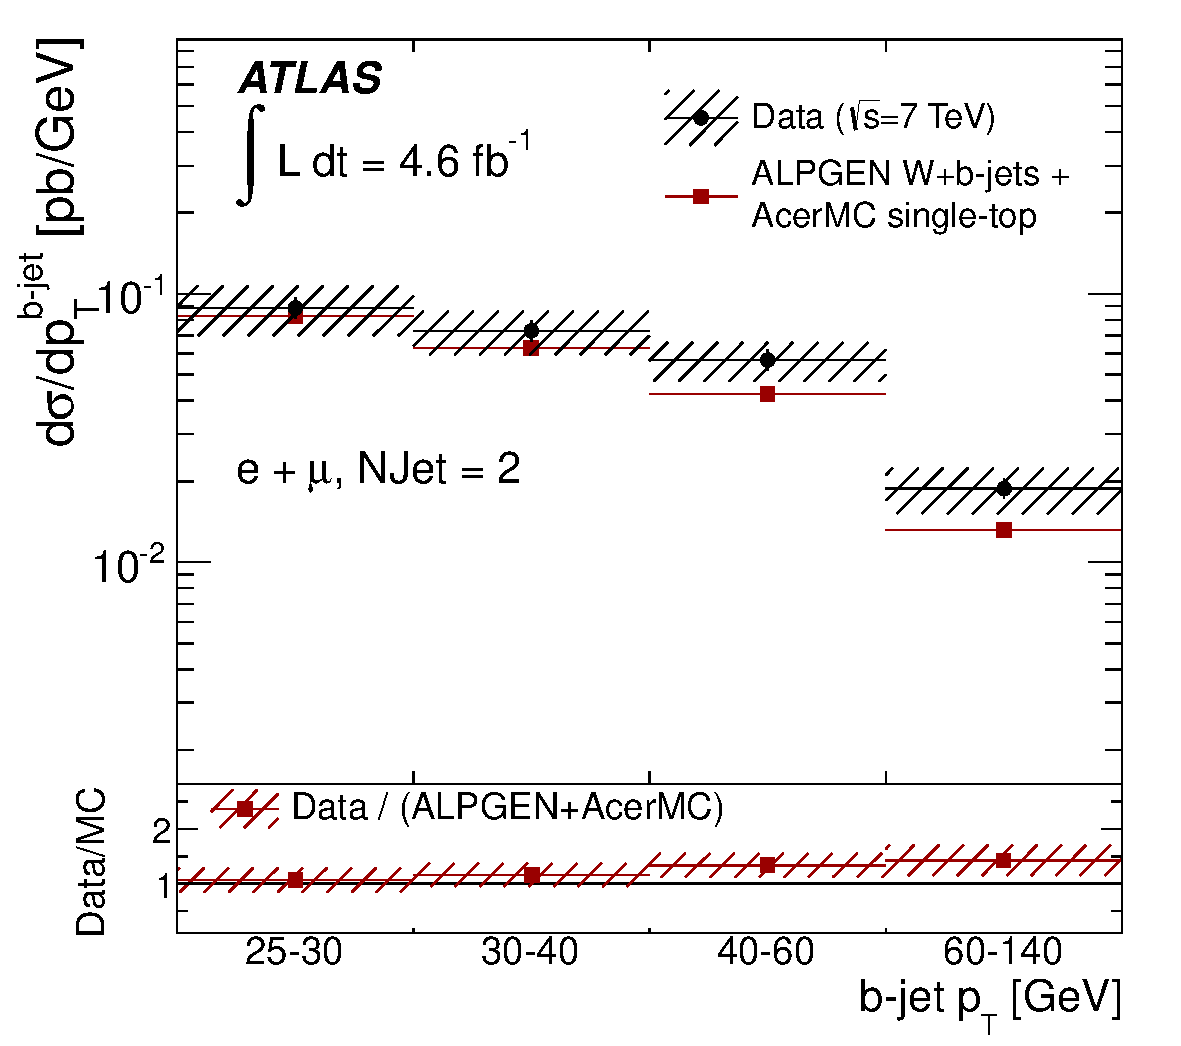
\includegraphics[width=0.48\textwidth]{fig_09b.pdf}
}
\caption{\label{fig:wb}
Measured differential $W+b$-jets cross-section without single-top subtraction as a function of the transverse momentum of the $b$-jet, in the case where the $b$-jet is the only jet in the fiducial region (a) or when there is an additional jet (b). The cross sections are obtained by combining the electron and muon channels. The measurements are compared to the sum of seperate $W+b$-jets and single-top predictions 
%obtained using ALPGEN interfaced to HERWIG and JIMMY and scaled by a NNLO inclusive $W$ normalization factor, and ACERMC interfaced to PYTHIA and scaled to a NLO single-top cross-section. 
The ratios between measured and predicted cross-sections are also shown. From~\protect\cite{Aad:2013vka}.}
\end{figure}

\begin{figure}%[htbp!]
\centering
\subfloat{
	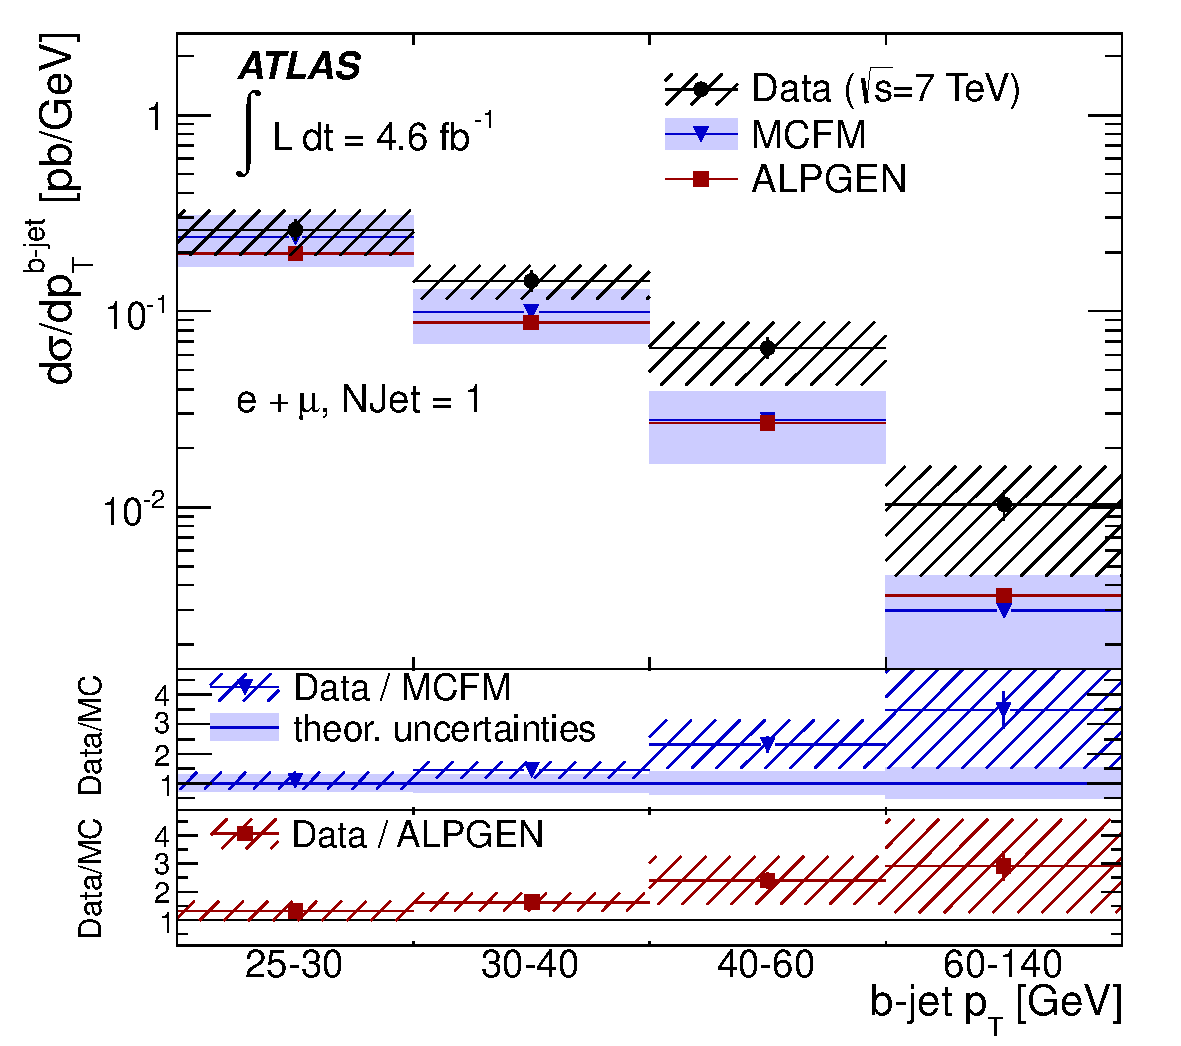
\includegraphics[width=0.48\textwidth]{fig_08a.pdf}
}
\subfloat{
	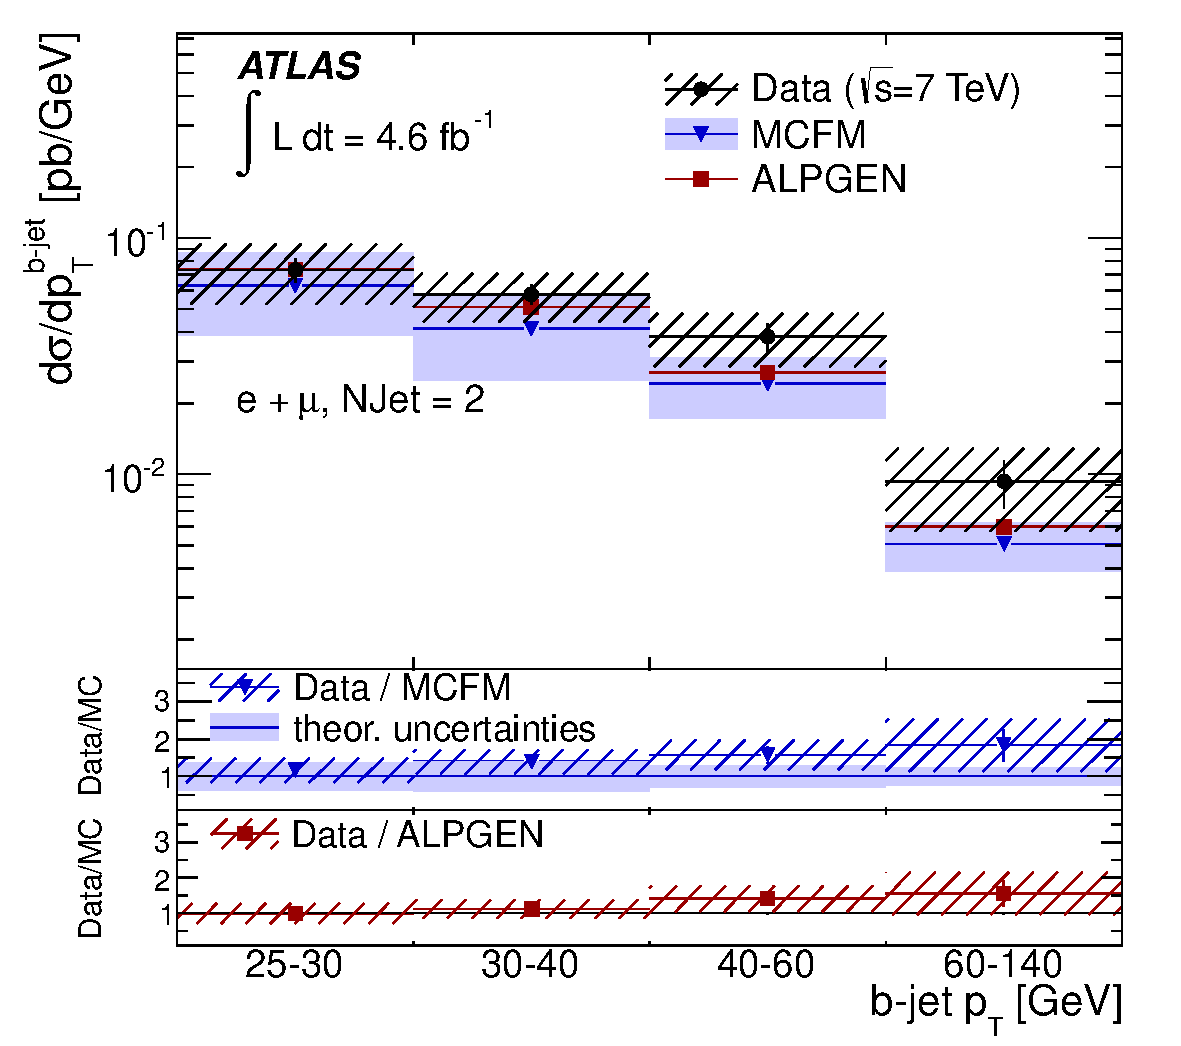
\includegraphics[width=0.48\textwidth]{fig_08b.pdf}
}
\caption{\label{fig:notop}
Measured differential $W+b$-jets cross-section after single-top subtraction as a function of the transverse momentum of the $b$-jet, in the case where the $b$-jet is the only jet in the fiducial region (a) or when there is an additional jet (b). The cross sections are obtained by combining the electron and muon channels. The measurements are compared to the a calculation of $W+b$-jet production in the absence of top quark propagators.
%obtained using ALPGEN interfaced to HERWIG and JIMMY and scaled by a NNLO inclusive $W$ normalization factor, and ACERMC interfaced to PYTHIA and scaled to a NLO single-top cross-section. 
The ratios between measured and predicted cross-sections are also shown. From~\protect\cite{Aad:2013vka}.}
\end{figure}

Several things may be noted:
\begin{itemize}
\item In neither case does the theory describe the data especially well. This is a challenging
final state to predict and the theory is likely to be superseded by more sophisticated and 
accurate predictions in future. This strongly mitigates against embedding in a dependency 
on the theory in the experimental analysis - as is the case if the background is subtracted at detector-level - 
and is a strong motivation for the unsubtracted version of the measurement.
\item The contributions from diagrams with and with top are comparable (compare the cross section in the lowest $p_T$ bin, 
for example).
\item The uncertainties on the unsubtracted version are smaller.
\end{itemize}

Integrated over $p_T$, the unsubstracted fiducial cross section is
$9.6 \pm 0.2 (stat) \pm 1.7 (syst)$ pb, a fractional systematic uncertainty of 18\%.
The corresponding subtracted measurement is 
$7.1 \pm 0.5 (stat) \pm 1.4 (syst)$ pb, a fractional systematic uncertainty of 20\%
- a small but noticeable effect decrease in precision. Looking in more detail, the main contributions 
to the systematic errors are
\begin{itemize}
\item Jet energy scale: 10-50\%
\item Modelling of initial and final state QCD radiation on these two processes and on $t\bar{t}$: 2-30\%
\item $b$-tagging 1-8\%
\item MC modelling (but only of the $Wb$ “signal”) 2-8\%
\end{itemize}
The fact that jet energy scale dominates masks, to a large extent, the effect of the modelling uncertainties introduced by
the background subtraction.
The uncertainty due to the modelling of QCD radiation varies a lot with jet $p_T$. 
This is exactly the kind of model dependence which one would expect to increaase if a theory-based background
subtraction is made, and indeed, in the highest $p_T$ bin the systematic uncertainty goes from 16\% before subtraction 
to 54\% after it (Compare Table~4 with Table~9 of Ref.\cite{Aad:2013vka}.) 

{\bf To be included if UCL students manage to make the plots}
{\it As the analysis is available in Rivet, it is relatively straightforward to repeat the comparison
with more modern MC calculations (Herwig++ and Sherpa) and to modify the analysis for 13~TeV collisions.
See plots, and discuss them.}

\section{$WWb\bar{b}$ production}

\section{Conclusions}\label{sec:conclusions}

\section*{Acknowledgments}


\bibliographystyle{h-physrev4}
\bibliography{backsub}

\end{document}


